%%%%%%%%%%%%%%%%%%%%%%%%%%%%%%%%%%%%%%%%%%%%%%%%%%%%%%%%%%%%%%%%%%%%%%%%
%                                                                      %
% LaTeX, FIIW thesis template                                          %
% 28/11/2014 v1.2                                                      %
%                                                                      %
%%%%%%%%%%%%%%%%%%%%%%%%%%%%%%%%%%%%%%%%%%%%%%%%%%%%%%%%%%%%%%%%%%%%%%%%
\documentclass[11pt,a4paper]{report}
% Indien je je thesis recto-verso wil afdrukken gebruik je onderstaande opties i.p.v. bovenstaande
%\documentclass[11pt,a4paper,twoside,openright]{report}

\usepackage[a4paper,left=3.5cm, right=2.5cm, top=3.5cm, bottom=3.5cm]{geometry}
\usepackage[dutch]{babel}
\usepackage{graphicx}
\usepackage[latin1]{inputenc}           % om niet ascii karakters rechtstreeks te kunnen inputten
%\usepackage[utf8]{inputenc}            % commentarieer deze regel uit als je utf8 encoded files gebruikt in plaats van latin1
\usepackage{natbib}
\usepackage{listings}             		% voor het weergeven van broncode
\usepackage{verbatim}					% weergeven van code, commando's, ...
\usepackage{hyperref}					% maak PDF van de thesis navigeerbaar
\usepackage{url}						% URL's invoegen in tekst met behulp van \url{http://}
\usepackage[small,bf,hang]{caption}     % om de captions wat te verbeteren
\usepackage[final]{pdfpages}            % gebruikt voor het invoegen van het artikel in pdf-formaat
\usepackage{pslatex}					% andere lettertype's dan de standaard types
\usepackage{lipsum}
\usepackage{sectsty}					% aanpassen van de fonts van sections en chapters
%\usepackage[nottoc,numbib]{tocbibind}	% Bibliography mee in de ToC

\allsectionsfont{\sffamily}
\chapterfont{\raggedleft\sffamily}

\usepackage{float}                      % De optie H voor de plaatsing van figuren op de plaats waar je ze invoegt. bvb. \begin{figure}[H]
%\usepackage{longtable}					% tabellen die over meerdere pagina's gespreid worden
%\usepackage[times]{quotchap}           % indien je fancy hoofdstuktitels wil
%\usepackage[none]{hyphenat}
%\usepackage{latexsym}
%\usepackage{amsmath}
%\usepackage{amssymb}

% MFA: zet zoekpad voor figure
\graphicspath{{fig/}}

\usepackage{fiiw}
% \usepackage{fiiw_denayer_eng} % For the english version (also change last page at the bottom of this file!

%door onderstaande regels in commentaar te zetten, of op false, kan je pagina's weglaten
%bijvoorbeeld het weglaten van een voorwoord, lijst met symbolen, ...
%%%%%%%%%%%%%%%%%%%%%%%%%%%%%%%%%%%%%%%%%%%%%%%%%%%%%%%%%%%%%%%%%%%%%%%%%%%%%%%%%%%%%%%%
%voorwoord toevoegen?
\acknowledgementspagetrue
\acknowledgements{voorwoord}			%.tex file met daarin het voorwoord

%samenvatting toevoegen
\summarypagetrue
\summary{samenvatting}					%.tex met daarin de samenvatting

%abstract toevoegen?
\abstractpagetrue
\abstracts{abstract}					%.tex file met daarin het abstract
%lijst van figuren toevoegen?
\listoffigurespagetrue
%lijst van tabellen toevoegen?
\listoftablespagetrue
%lijst van symbolen toevoegen?
\listofsymbolspagetrue
\listofsymbols{symbolen}				%.tex file met daarin de lijst van symbolen



%informatie over het eindwerk, de promotor, ...
%%%%%%%%%%%%%%%%%%%%%%%%%%%%%%%%%%%%%%%%%%%%%%%
\opleiding{naam opleiding}
\afdeling{afstudeerrichting vermelden}

\campus{groupteng} %denayer,denayereng,geel,geeleng,gent,ghenteng,groept,groupteng,brugge,brugeseng

\title{Titel masterproef}
\subtitle{Ondertitel (facultatief)}
% \author{naam student}
\forenameA{Jan}
\surnameA{Janssens}

% l
\forenameB{Peter}
\surnameB{Peeters}

\academicyear{2017 - 2018}

\promotorA[Promotor]{Prof. dr. ir. Grote Baas}
\promotorB[Co-promotor(en)]{Prof. dr. ir. Andere Baas}
\promotorC[]{dr. Bedrijf Baas (Bedrijf)}

\begin{document}
\selectlanguage{dutch}
% \selectlanguage{english} % For the english version
\preface

%%%%%%%%%%%%%%%%%%%%%%%%%%%%%%%%%%%%%%%%%%%%%%%%%%%%%%%%%%%%%%%%%%% 
%                                                                 %
%                            CHAPTER                              %
%                                                                 %
%%%%%%%%%%%%%%%%%%%%%%%%%%%%%%%%%%%%%%%%%%%%%%%%%%%%%%%%%%%%%%%%%%% 

\chapter{Vormelijke richtlijnen van de scriptie}

\section{Verplichte onderdelen en volgorde in de scriptie}

De masterproefscriptie bevat volgende onderdelen

\begin{itemize}
\item	Voorkaft met titelblad
\item Herhaling titelblad
\item	Bladzijde met verplichte tekst copyright
\item	Voorwoord
\item	Samenvatting
\item	Abstract
\item	Inhoudstafel
\item	Symbolenlijst
\item	Masterproeftekst
\item	Referentielijst
\item	Bijlagen
\item	Achterkaft met gegevens van de campus
\end{itemize}

\section{Lay-out}
De scriptie is standaard in het Nederlands, maar mag in het Engels geschreven worden mits motivatie. 

Dit document is opgesteld volgens de vereiste lay-out van de faculteit. Hieronder volgen een aantal specifieke richtlijnen die ook in de template\footnote{Deze template dient gebruikt te worden in combinatie met LaTeX. Voor meer informatie over de installatie en het gebruik hiervan, wordt doorverwezen naar \href{https://www.latex-project.org/}{deze website} verwerkt zijn.}

\subsection{Papierformaat en bladspiegel}
Deze LaTeX-template is opgesteld volgens de geldende regels van de faculteit. Het is dus niet toegalaten zelf aanpassingen aan de stijl ervan te doen. Bij voorkeur wordt de thesis recto-verso afgedrukt.

\subsection{Titelblad}
Volg nauwgezet de aanwijzigen in deze template voor het opstellen van het titelblad.

Is een masterproef uitgevoerd onder \textit{embargo}, dan wordt dit expliciet vermeld op het titelblad (onder voorbehoud van goedkeuring van de fPOC). De cover wordt geprint in kleur op wit papier. Indien meerdere studenten samen een masterproef realiseren, worden de namen alfabetisch op achternaam weergeven op het titelblad door deze in de juiste volgorde in de template in te vullen. Een student die een Nederlandstalige opleiding volgt en de toelating heeft gekregen om zijn masterproefscriptie in het Engels te schrijven, moet het Nederlandstalige titelblad nog steeds gebruiken. De titel zelf is dan wel in het Engels.

%%%%%%%%%%%%%%%%%%%%%%%%%%%%%%%%%%%%%%%%%%%%%%%%%%%%%%%%%%%%%%%%%%% 
%                                                                 %
%                            CHAPTER                              %
%                                                                 %
%%%%%%%%%%%%%%%%%%%%%%%%%%%%%%%%%%%%%%%%%%%%%%%%%%%%%%%%%%%%%%%%%%% 

\chapter{Structuur van de masterproeftekst}

\section{Opdeling in hoofdstukken}
De masterproeftekst vormt de kern van de scriptie. De tekst wordt logisch opgedeeld in een aantal hoofdstukken. Het eerste hoofdstuk is altijd een inleiding, het tweede en eventueel derde de literatuurstudie of een \textit{state of the art}, gevolgd door een hoofdstuk dat de methodologie beschrijft. De volgende hoofdstukken bevatten de elementen van het eigen onderzoek. Het laatste hoofdstuk bevat de algemene besluiten van de masterproef. Elk hoofdstuk vormt een afgerond geheel (m.a.w. met inleiding en conclusie!).

\section{Verdere onderverdeling binnen een hoofdstuk}
De tekst wordt onderverdeeld in logische paragrafen met een aangepaste nummering. De nummering van de onderliggende delen van een hoofdstuk bevat begint steeds met het hoofstuknummer en gaat maximum tot drie subniveaus. 
Volgende onderverdeling wordt gebruikt:

\section{Dit is een voorbeeld van een sectie}
\subsection{Dit is een voorbeeld van een subsectie}
\subsubsection{Dit is een voorbeeld van een subsubsectie}
\paragraph{Dit is een voorbeeld van een paragraaf}
%%%%%%%%%%%%%%%%%%%%%%%%%%%%%%%%%%%%%%%%%%%%%%%%%%%%%%%%%%%%%%%%%%% 
%                                                                 %
%                            CHAPTER                              %
%                                                                 %
%%%%%%%%%%%%%%%%%%%%%%%%%%%%%%%%%%%%%%%%%%%%%%%%%%%%%%%%%%%%%%%%%%% 
\chapter{Implementatie van Herkenning en detectie op mobiel platform}
Dit hoofdstuk gaat over het implementeren van deep learning herkenningssystemen en detectiesystemen op een mobiel platform.
Bij het uitvoeren van een neuraal netwerk op een mobiel apparaat zal men rekening moeten houden met gelimiteerde rekenkracht en het beschikbaar geheugen.
Het uitvoeren van de vele berekeningen en geheugen operaties zal ook invloed hebben op de batterij van het mobiel toestel.
Eerst zullen we een aantal frameworks bespreken waarmee we neurale netwerken kunnen ontwerpen, trainen en deployen.
Vervolgens zullen we een aantal bibliotheken bespreken die ons extra hulpmiddelen geven om detectiesystemen mee te ontwerpen.
Dan gaan we een aantal frameworks bespreken die specifiek ontworpen zijn voor mobiele implementaties.
Als laatste gaan we een aantal optimalisatietechnieken bespreken waarmee we het neurale netwerk verder kunnen optimaliseren.
Er zal voornamelijk gefocust worden op Android implementaties.

\section{Frameworks}
Om machine learning modellen te ontwerpen en te trainen kan er gebruik gemaakt worden van frameworks.
Deze frameworks geven de programmeur een set van tools die hem in staat stelt om op een overzichtelijke en flexibele manier deep learning modellen te ontwerpen en trainen.
TensorFlow (\cite{abadi_tensorflow_2016}) en PyTorch (\cite{li_PyTorch_2020}) zijn de twee voornaamste frameworks om neurale netwerken te ontwerpen.
Veel van de tools en bibliotheken die we gebruiken om complexere herkenningssystemen en detectiesystemen te ontwerpen worden bovenop deze frameworks gebruikt.
Vanwege hun populariteit gaan we de twee frameworks bespreken en gaan we kijken welke mogelijkheden elk framework heeft.

\subsection{TensorFlow}
TensorFlow (\cite{abadi_tensorflow_2016}) is ontworpen door Google en is een open source framework voor machine learning implementaties dat focust op het ontwerpen, trainen en deployen van neurale netwerken.
Ook ondersteund TensorFlow meerdere programmeertalen zoals: Python, Java en C.

%Keras
Door de introductie van de Keras API (\cite{chollet2015keras}) is TensorFlow meer gebruiksvriendelijk.
Keras is een framework dat bovenop TensorFlow gebruikt kan worden en waarmee we machine learning modellen kunnen ontwerpen op een overzichtelijke manier.
Het idee van Keras is om zo snel mogelijk van een idee naar een toepassing te gaan.
Zo heeft TensorFlow een gebruiksvriendelijk API voor eenvoudige projecten en meer uitgebreide tools voor complexe projecten.
Ondertussen is Keras ge\"integreerd met het TensorFlow framework.

%Programmeurs kunnen op een grafische manier de operaties voorstellen die moeten worden uitgevoerd.
%Hierbij bestaat de grafische voorstelling uit nodes, waarbij elke node een wiskundige operatie is.
%Zo krijgt de programmeur een duidelijk overzicht over de gehele toepassing.
%Door gebruik te maken van TensorBoard (\cite{tensorflow2015-whitepaper}) kan data op een flexibele manier gevisualiseerd worden tijdens het ontwerpen van een machine learning model.
%TensorFlow biedt ook goede ondersteuning op gebied van deployment van een model.
%De grootte community achter zich heeft, omdat dit een veel gebruikt framework is.

%TensorFlow Object Detection API
De TensorFlow Object Detection API (\cite{tensorflow2015-whitepaper}) is een open source framework dat bovenop TensorFlow werkt. 
Het maakt het voor de programmeur eenvoudiger om detectiemodellen te ontwerpen, trainen en deployen.
Deze API voorziet een set van meer dan 40 modellen voorgetraind op de COCO dataset waarop de programmeur verder kan bouwen. 
De COCO dataset is een grote dataset voor objectdetectie en segmentatie gepubliceerd door Microsoft (\cite{lin2015microsoft}).
De API heeft voorgetrainde detectiemodellen van de volgende architecturen: CenterNet (\cite{duan_centernet_2019}) RetinaNet (\cite{lin_focal_2018}), EfficientDet (\cite{tan_efficientdet_2020}), SSD (\cite{liu_ssd_2016}) en Faster-RCNN (\cite{ren_faster_2016}).
%De Object Detection API kan ook ge\"importeerd worden in Android studio, waardoor het TFLite model op een eenvoudige manier ge\"implementeerd kan worden op een mobiele applicatie.	

\subsection{PyTorch}
PyTorch (\cite{li_PyTorch_2020}) is ontworpen door Facebook en wordt zoals TensorFlow ook gebruikt om machine learning modellen te ontwerpen, trainen en deployen.
Dit is een python gebaseerd framework dat focust op flexibiliteit.
Door zijn flexibiliteit is het eenvoudig om nieuwe functionaliteiten toe te voegen door bestaande code aan te passen of nieuwe code toe te voegen.
%Zoals TensorFlow kan het model worden voorgesteld op een grafische manier die bestaat uit nodes en waarbij elke node een operatie is.
%PyTorch maakt gebruik van externe tools zoals TensorBoard om data te visualiseren.
%PyTorch wordt voornamelijk gebruikt om te experimenteren met neurale netwerken.
%Bedrijven en onderzoekers gebruiken dit framework vooral om een CNN experimenteel op te bouwen en te trainen.
%dynamisch model ontwerp

Via de Torchvision bibliotheek (\cite{Facebook_PyTorch_2017}) die deel uitmaakt van het PyTorch project, heeft de programmeur toegang tot een set van hulpmiddelen om een deep learning model op te bouwen.
Torchvision bevat populaire datasets, netwerk architecturen en technieken voor afbeelding transformaties.
Voor objectdetectie biedt Torchvision ondersteuning voor de Faster-RCNN (\cite{ren_faster_2016}), RetinaNet (\cite{lin_focal_2018}), SSD (\cite{liu_ssd_2016}) en SSDlite (\cite{sandler_mobilenetv2_2019}) architecturen.
Van deze architecturen zijn er een aantal voorgetrainde modellen terug te vinden in de Torchvision bibliotheek.
Via transfer learning is de programmeur dan in staat om een eigen detectiemodel te trainen.

\section{Objectdetectie bibliotheken} \label{lib}
Er zijn heel wat bibliotheken die de programmeur kan importeren om een detectiesysteem te ontwerpen en te trainen.
Deze bibliotheken geven de programmeur extra hulpmiddelen om de complexiteit van het process te verminderen en de code overzichtelijk te maken.
De bibliotheken werken bovenop TensorFlow of PyTorch en geven de programmeur toegang tot een groter aantal verschillende objectdetectoren en voorgetrainde modellen.

\subsection{MMDetection}
MMDetection voorgesteld door \cite{chen_mmdetection_2019} maakt deel uit van OpenMMLab en is een open source objectdetectie toolbox gebaseerd op PyTorch.
Deze bibliotheek is specifiek ontworpen voor objectdetectie taken.
MMDetection ondersteund ook 48 verschillende detectiemethodes zoals: YOLO (\cite{redmon_you_2016}), Faster R-CNN (\cite{ren_faster_2016}), en SSD (\cite{liu_ssd_2016}).
Van al deze architecturen samen heeft de programmeur toegang tot meer dan 200 voorgetrainde modellen.
Een belangrijk aspect van MMDetection is dat het eenvoudige componenten bevat van verschillende detectie architecturen.
Door deze componenten te combineren kan de programmeur een nieuw detectiemodel ontwerpen.

Doordat al de bounding box en masker operaties worden uitgevoerd op GPU's heeft MMDetection een grote trainingssnelheid.
MMDetection biedt zelf geen ondersteuning om een bestaand model te optimaliseren naar een model voor mobiel gebruik.
%Omdat een MMDetection model operaties kan bevatten die een Pytorch model niet ondersteund, kan het zijn de de optimalisatie naar PyTorch mobile niet lukt.
%Dus dit model zal geconverteerd moeten worden naar een framework waarbij het optimaliseren naar een mobiel model wel mogelijk is.
%suports COCO en VOC style datasets

\subsection{Detectron2}
Detectron2 (\cite{wu2019detectron2}) is een bibliotheek ontworpen door Facebook die segmentatie en detectie algoritmes ondersteunt.
Zoals MMDetection werkt Detectron2 bovenop Pytorch en kan het netwerk getraind worden op een GPU.
%Volgens de Detectron2 documentatie heeft Detectron2 een betere trainingssnelheid dan MMDetection.
%Detectron2 verwerkt 62 afbeeldingen/s en MMDetection 53 afbeeldingen/s bij het trainen van een Mask R-CNN detector.
Via Modular, extensible design kan Detectron2 specifieke modules toevoegen aan bijna elk deel van een detectiesysteem.
Detectron2 bevat meer dan 80 voorgetrainde modellen waarop de programmeur verder kan bouwen.
Voor objectdetectie ondersteund Detectron2 zes verschillende standaardmodellen.
Ondertussen heeft Detectron2 D2Go als uitbreiding gekregen dat ondersteuning biedt voor objectdetectie voor mobiele toepassingen.

\subsection{GluonCV}
GluonCV (\cite{guo_gluoncv_2020}) is een bibliotheek die implementaties levert voor enkele van de State-of-the-art deep learning modellen.
Voor objectdetectie biedt GluonCV ondersteuning voor vier detectiemodellen: SSD (\cite{liu_ssd_2016}), Faster-RCNN (\cite{ren_faster_2016}), YoloV3 (\cite{redmon_yolov3_2018}) en CenterNet (\cite{duan_centernet_2019})
Deze bibliotheek is ontworpen om snel prototypes en onderzoeksidee\"en te leveren voor onderzoekers.
Dit doet GluonCV door de programmeur toegang te geven tot 170 voorgetrainde modellen, die hertraind kunnen worden voor een specifiek doel.
Met behulp van een API die de complexiteit van het implementeren minimaliseert.
GluonCV biedt ondersteuning voor PyTorch en MXNet om deep learning modellen te ontwerpen en trainen.
De GluonCV documentatie bevat meer informatie voor MXNet dan voor PyTorch.
MXNet is een framework zoals PyTorch en TensorFlow om neurale netwerken te ontwerpen, trainen en deployen (\cite{chen_mxnet_2015}).

\subsection{ImageAI}
ImageAI (\cite{martins_imageai_2021}) is een eenvoudig te gebruiken Python bibliotheek die de programmeur in staat stelt om State-of-the-art AI feautres te implementeren.
Het doel van deze bibliotheek is om met enkele lijnen code een objectdetector te trainen.

\begin{python}
from imageai.Detection.Custom import DetectionModelTrainer

trainer = DetectionModelTrainer() # init
trainer.setModelTypeAsYOLOv3()	# model type
trainer.setDataDirectory('path_to_dataset_dir') # dataset dir
#training configuratie(lijst met labels, batch size, aantal epochs, voorgetraind model)
trainer.setTrainConfig(object_names_array=["labels"], batch_size=4, num_experiments=200, train_from_pretrained_model="pretrained-yolov3.h5")
trainer.trainModel()
\end{python}

Deze bibliotheek levert tools voor herkenning, objectdetectie en videoanalyse.
ImageAI geeft de programmeur toegang tot voorgetrainde detectiemodellen van RetinaNet (\cite{lin_focal_2018}) , YoloV3 (\cite{redmon_yolov3_2018}) en TinyYOLOv3 (\cite{Gai_TinyV3_2021}) getraind met de COCO dataset.
Deze bibliotheek werkt bovenop TensorFlow en maakt sinds juni 2021 gebruik van een PyTorch backend.
Ook deze bibliotheek geeft de programmeur de mogelijkheid om nieuwe modellen te trainen om specifieke objecten te detecteren.

\section{Open Neural Network Exange (ONNX)}
\cite{onnx_onnx_2017} biedt de mogelijkheid om deep learning model te exporteren naar een ander framework.
Hierbij converteren we een bestaand model naar een ONNX model.
Dit model kan op zijn beurt geconverteerd worden naar het gewenste framework (figuur: \ref{fig:onnx}).
Volgens de website van ONNX zijn er momenteel 23 frameworks die naar het ONNX framework geconverteerd kunnen worden, waaronder PyTorch en TensorFlow.
Deze modellen kunnen we dan converteren naar een framework dat het model kan implementeren op een mobiel apparaat.
Voor deze masterproef waarin een bestaand model ontworpen is in een bepaald framework, zal ONNX een belangrijke rol spelen.
Op deze manier kunnen we een bestaand model implementeren met een framework dat mobiele implementatie ondersteund.

ONNX definieert een aantal gemeenschappelijke sets van operaties en bouwblokken genaamd opsets.
Deze opsets bevatten operaties die compatibel zijn met operaties van andere frameworks.
Bij het converteren naar een ONNX model zullen de operaties die uitgevoerd worden in een bepaald framework vervangen worden door een ONNX equivalent gedefinieerd in een opsetversie.
ONNX vernieuwt de opsets regelmatig, zo zal bij elke opsetversie de operaties worden aangepast waardoor er operaties bijkomen, wijzigen en wegvallen.
Niet elk framework ondersteunt dezelfde opsetversie en dit zou tijdens het exporteren naar ONNX voor problemen kunnen zorgen.
Dit is omdat een bepaalde operatie van een framework geen ONNX-equivalent zou kunnen hebben.
Voor elke bibliotheek/framework is het aangeraden om dezelfde opsetversie te implementeren.

\begin{figure}[!ht]
    \centering
 	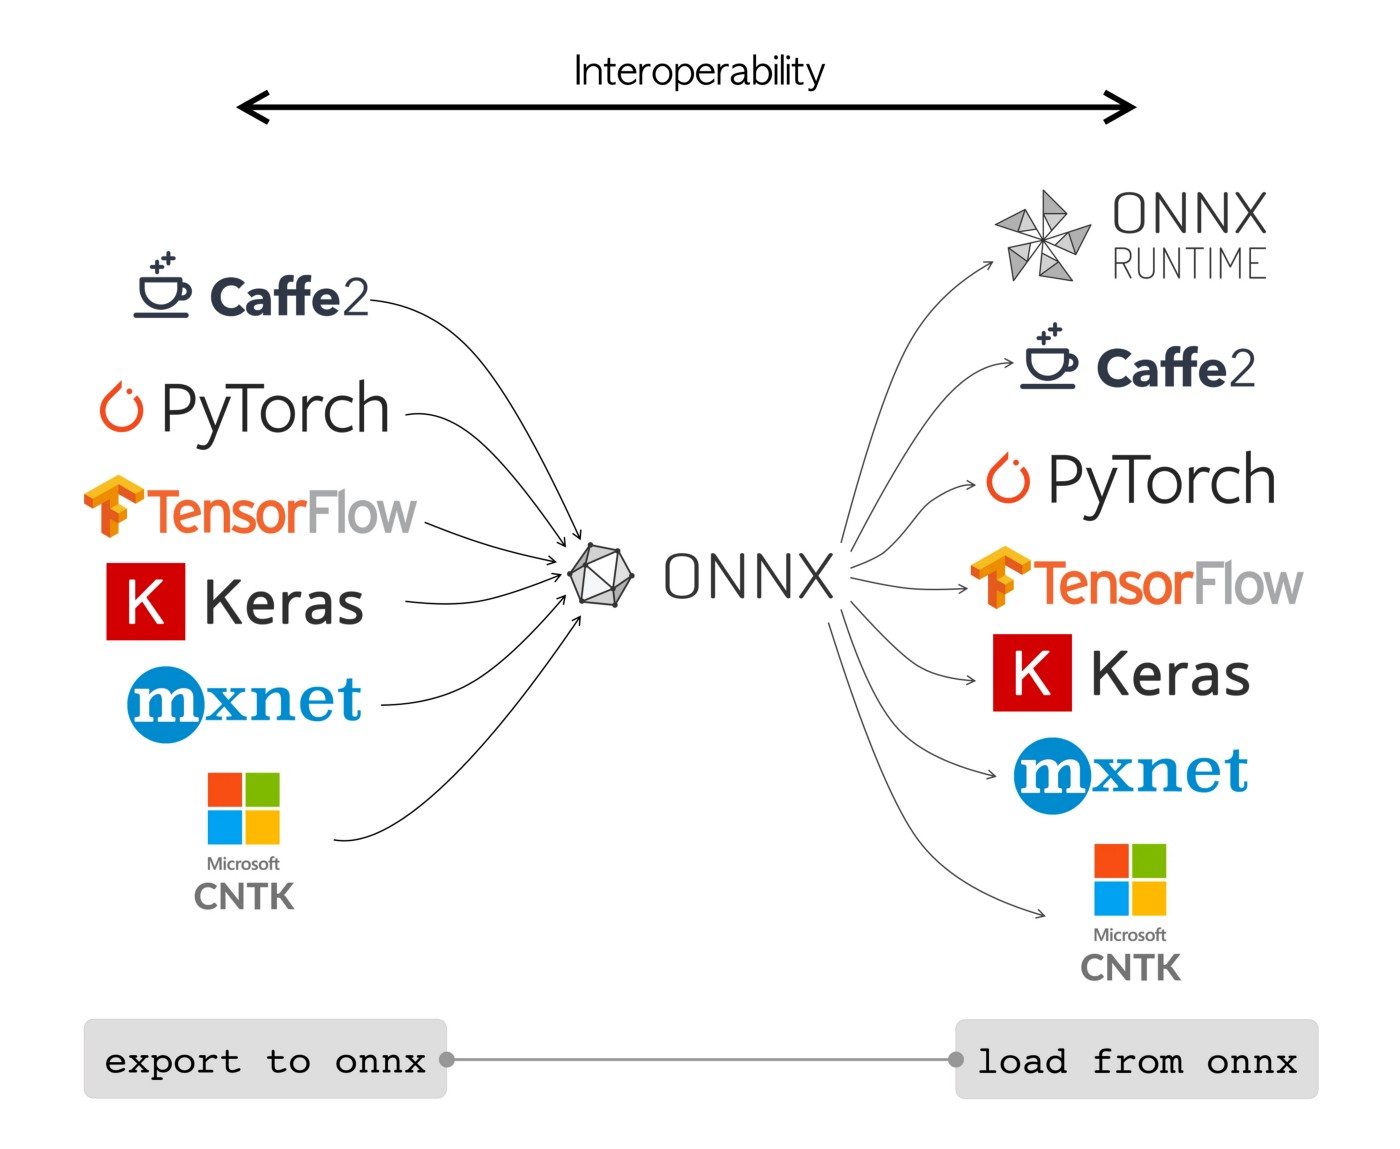
\includegraphics[width=0.7\linewidth]{fig/onnx.jpeg}
 	\caption{Een weergave van de voornaamste frameworks die naar ONNX kunnen exporten en die een ONNX model kunnen importeren.}
 	\label{fig:onnx}
\end{figure}

\subsection{TensorFlow naar ONNX conversie}
Om een TensorFlow model naar ONNX formaat te exporteren wordt er gebruik gemaakt van de tf2onnx bibliotheek (\cite{onnx_tf2onnx_2021}).
Via de volgende lijn code kan de convert functie worden opgeroepen uit de tf2onnx bibliotheek.

\begin{python}
python -m tf2onnx.convert --saved-model <directory van opgeslagen model> 
		--output <onnx output file> --opset <opsetversie>
\end{python}

%\begin{lstlisting}[language=Python, caption=Converteren van TensorFlow model naar ONNX model]
%!python -m tf2onnx.convert --saved-model <directory van opgeslagen model> 
%		--output <onnx output file> --opset <opset versie>
%\end{lstlisting}

De conversie van TensorFlow naar ONNX wordt voor opsetversie 9 tot 15 ondersteund en getest.
Opsetversie 6 tot 8 zou ook ondersteund moeten worden maar hier zijn geen testen voor.
Bij de conversie wordt opsetversie 9 standaard gebruikt.
Voor een meer recente opsetversie moet de opsetversie specifiek worden meegegeven via bovestaande code met de optie '--opset'.
In de Tf2onnx documentatie is een lijst terug te vinden met Tensorflow operaties die ONNX ondersteund.
Als het TensorFlow model operaties bevat die niet herkend worden door onnxruntime, dan is het mogelijk om deze operaties mee te geven met de conversie functie.
%Hoe
De TensorFlow naar ONNX conversie bestaat uit de volgende stappen: 

\begin{itemize}
	\item De converter verwacht een Protobuf bestand (\cite{Google_protocol_2014}) als input omdat de converter constante variabelen verwacht van het opgeslagen model. Protobuf is een serieel formaat dat platformonafhankelijk is.
	\item Het TenserFlow protobuf formaat wordt geconverteerd naar het ONNX protobuf formaat zonder rekening te houden met specifieke operaties.
	\item De converter identificeert operaties en vervangt deze met het ONNX equivalent.
	\item Er wordt gekeken naar specifieke operaties die niet automatisch zijn vervangen door een ONNX equivalent. Bijvoorbeeld operatie relu6 wordt niet door ONNX ondersteund, maar kan vervangen worden door verschillende ONNX operaties te combineren.
	\item Het huidige ONNX model wordt verder geoptimaliseerd door bijvoorbeeld operaties samen te voegen of onnuttige operaties te verwijderen.
\end{itemize}

\subsection{PyTorch naar ONNX conversie}
De tools om een PyTorch model te converteren naar een ONNX model maken standaard deel uit van PyTorch.
Zo kan via de volgende lijn code een PyTorch model ge\"exporteerd worden naar ONNX.

\begin{python}
torch.onnx.export(model, args, 'test.onnx')
\end{python}

De verplichte inputs nodig voor het uitvoeren van deze functie zijn: het PyTorch model, een set van inputargumenten en een output bestand.
De set van inputargumenten bestaat uit een tuple van inputs of een dictionary die de input parameters van het model geeft.
Bij het uitvoeren van torch.onnx.export zal de functie het model omzetten in een TorchScript model dat wordt besproken in paragraaf \ref{trace}.
Hierbij zal het model worden uitgevoerd en zullen al de uitgevoerde operaties bewaard worden.
De inputargumenten meegegeven met de export functie zullen gebruikt worden als input voor de trace functie.
De operaties van het TorchScript model zullen dan vervangen worden door hun ONNX equivalent.
De PyTorch documentatie bevat een lijst met al de operaties die ondersteund worden voor het uitvoeren van de export functie naar ONNX.

Het is mogelijk om operaties die niet in deze lijst staan toe te voegen aan de PyTorch bron code als de operatie ondersteund wordt door ONNX.
Dit doen we door de operator te registreren in de native\_functions.yaml file die terug te vinden is in de volgende folder van de PyTorch bron code: pytorch/aten/src/ATen/native (\cite{pytorch_atensrcatennative_2021}).
Vervolgens moet in dezelfde folder de functie worden geschreven in een nieuwe C++ file.
In deze folder is ook meer informatie beschikbaar voor het toevoegen van niet ondersteunde operaties.
%Als er gewerkt wordt met de voorgetrainde modellen uit de TorchVision bibliotheek dan is het model exporteerbaar naar ONNX tenzij het model geoptimaliseerd is via quantisatie.

\section{Frameworks voor mobiele implementatie}
Er zijn een aantal frameworks die de programmeur de mogelijkheid geven om een model te optimaliseren voor een mobiel platform.
Deze frameworks hebben bovendien een API ter beschikking die het mogelijk maakt om het geoptimaliseerd model te implementeren in een mobiele omgeving.
We focussen op Android implementaties, maar de optie voor IOS zal ook vermeld worden.
Niet elke framework voor mobiele implementatie voert de zelfde optimalisatietechnieken uit.
Dus het converteren van het standaardmodel naar het mobiele model zal voor elk framework een ander resultaat geven.
Sommige modellen zullen na het optimaliseren in een bepaald framework een kleinere bestandsgrootte hebben dan bij andere frameworks.
Deze frameworks zullen een model importeren van PyTorch, TensorFlow of ONNX.

\subsection{TensorFlow Lite (TFLite)} \label{tf}
Voor mobiele implementatie biedt TensorFlow de mogelijkheid om een TFLite model te ontwerpen (\cite{tensorflow2015-whitepaper}).
De meeste detectiemodellen ontworpen met TensorFlow Object Detection API zijn niet bedoeld om op mobiele apparaten te werken.
Maar TensorFlow Object Detection API heeft ondersteuning om SSD  (\cite{liu_ssd_2016}) en EfficientDet (\cite{tan_efficientdet_2020}) architecturen te exporteren naar een TFLite model.
%
TFLite zorgt ervoor dat het model een lage latency heeft en een kleine binaire bestandsgrootte.
Deze modellen kunnen ge\"implenteerd worden op zowel Android als IOS applicaties.
Via de TFLite ObjectDetector API kunnen we TFLite detectiemodellen eenvoudig implementeren in Android studio.
Het converteren kan eenvoudig worden uitgevoerd via de volgende lijnen code in Python.

\begin{python}
import tensorflow as tf

converter = tf.lite.TFLiteConverter.from_saved_model(saved_model_dir)
tflite_model = converter.convert()
\end{python}	

De TFLiteConverter neemt een TensorFlow model als input en op basis van dit model wordt een converterobject gegenereerd.
Het TFLite model is eigenlijk een geoptimaliseerde FlatBuffer (\cite{Google_flatbuffers_2014}), deze kan herkend worden door de .tflite extensie.
FlatBuffer is serialisatie bibliotheek waarbij het object niet verpakt wordt en dus rechtsreeks uitleesbaar is voor verdere toepassingen.
Omdat het FlatBuffer object rechtsreeks uitleesbaar is zorgt dit voor een optimale snelheid en een effici\"ent geheugengebruik.
Het FlatBuffer formaat is niet python afhankelijk en is bruikbaar over verschillende platformen zoals: C, Java en Python.
Tijdens de TFLite conversie worden er ook een aantal verdere optimalisaties uitgevoerd via Grappler (\cite{tensorflow2015-whitepaper}) om het model kleiner en sneller te maken.
Grappler is het standaard optimalisatie systeem van TensorFlow om automatisch het model te verbeteren.
Grappler voert een heel aantal optimalisatie uit, de volgende technieken zijn enkele van de voornaamste Grappler optimalisaties: 

\begin{itemize}
	\item Constant Folding optimizer: Is het vervangen van operaties door constanten, bij operaties waarvan de waardes niet veranderen tijdens de uitvoering.  
	\item Remapper optimizer: operaties  in het model worden samengevoegd tot \'e\'en operatie.
	\item Memory optimizer: Analyseert het geheugengebruik van operaties in het model en voegt bij zwaar geheugengebruik swap operaties toe tussen CPU en GPU.
	\item Pruning optimizer: het verwijderen van operaties in het model die geen invloed hebben op de output.
\end{itemize}

De TFLite bibliotheek ondersteund een gelimiteerd aantal operaties van de standaard TensorFlow operaties.
Hierdoor is het mogelijk dat bij complexere modellen de TFLite conversie niet altijd succesvol is, omdat een bepaalde TensorFlow operatie geen TFLite tegenhanger heeft.
De lijst met ondersteunde TFLite operaties is terug te vinden in de TFLite documentatie.
%%%%%%%%%%%%%%% iets zeggen over welke operaties
Het is mogelijk om TensorFlow operaties te gebruiken die niet ondersteund worden door TFLite door dit mee te geven met de TFLiteConverter.
Dit heeft als gevolg dat de TensorFlow Core bibliotheek mee ge\"implementeerd moet worden waardoor de bestandsgrootte van het TFLite model zal toenemen.

\begin{python}]
converter.target_spec.supported_ops = [
	tf.lite.OpsSet.TFLITE_BUILTINS, # laat TFLite operaties toe.
	tf.lite.OpsSet.SELECT_TF_OPS # laat standaard TenserFlow operaties toe.
  ]
\end{python}	

TFLite geeft ook de mogelijkheid om modellen te hertrainen via TFLite Model Maker (\cite{tensorflow2015-whitepaper}).
Hierbij kan er voor objectdetectie enkel gebruik gemaakt worden van een EfficientDet detector (\cite{tan_efficientdet_2020}).
Als EfficienDet voldoet aan de nodige specificaties en het is voldoende om dit netwerk te hertrainen, dan geeft TFLite model maker de mogelijkheid om een TFLite model te hertrainen met een eigen dataset.
Op deze manier kan de conversiestap overgeslagen worden.

\begin{figure}[!ht]
    \centering
 	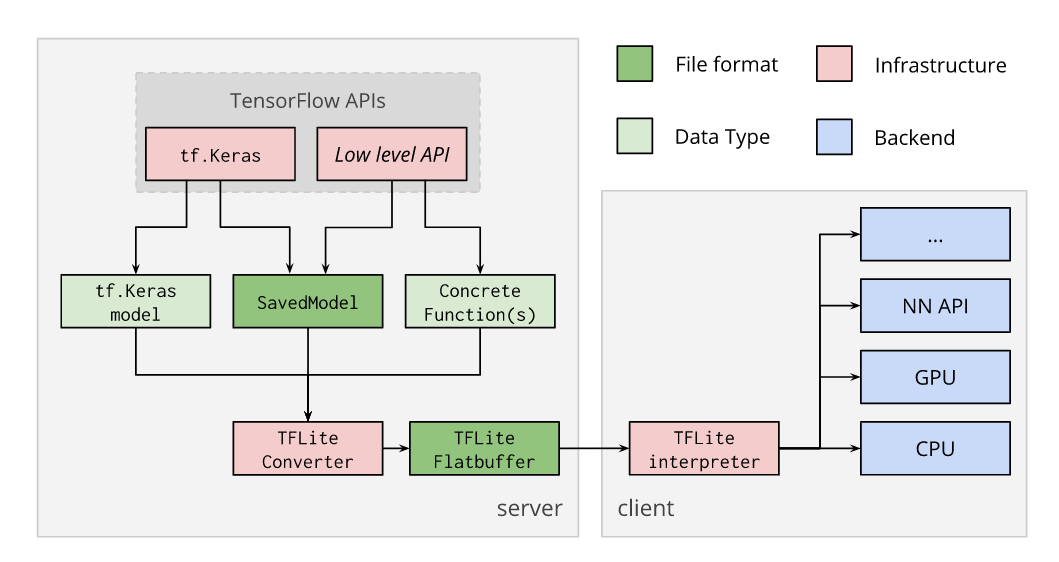
\includegraphics[width=0.7\linewidth]{fig/TFLite_workflow.png}
 	\caption{Implementatieflow van een TensorFlow model naar een mobiele implementatie. Aan de linker kant is te zien dat een TensorFlow model via de TFLite converter wordt omgezet in TFLite flatbuffer model.
	 Het TFLite flatbuffer model kan vervolgens ge\"implementeerd worden op een client toestel waar er gebruik gemaakt kan worden van verschillende hardware componenten}
 	\label{fig:tflite}
\end{figure}

Het framework geeft ook de mogelijkheid om TFLite model verder te verbeteren via hardwareacceleraties en modeloptimalisaties.
De modeloptimalisaties die TFLite ondersteunt zijn: weight pruning, kwantisatie en clustering.
Wat deze optimalisatietechnieken exact inhouden wordt later besproken in paragraaf \ref{optim}.
De kwantisatie optimalisatie kan als optie worden meegegeven aan de TFLiteConverter.
Weight pruning en clustering moeten uitgevoerd worden voordat het model geconverteerd wordt naar TFLite.

De uitvoering van het TFLite model dat normaal op de CPU wordt uitgevoerd, kan versneld worden door gebruik te maken van verschillende hardwarecomponenten die op het toestel aanwezig zijn.
Elk van deze hardwarecomponenten maakt gebruik van een eigen API waardoor er extra code moet worden geschreven specifiek voor elke hardwarecomponent.
De TensorFlow Lite Delegate API (\cite{tensorflow2015-whitepaper}) dient als een interface in de vorm van delegates voor deze componenten.
Deze delegates zorgen ervoor dat we geen specifieke API moeten implementeren voor een bepaalde hardwarecomponent. 
TFLite ondersteund meerdere delegates die kunnen geoptimaliseerd worden voor een specifiek platform.
Voor Android kunnen we gebruik maken van de GPU delegate en de Neural Network API (NNAPI) delegate.
De NNAPI (\cite{Android_NNAPI_2021}) is ontworpen om intensieve berekeningen uit te voeren op een Android apparaat.
Deze API wordt aangeroepen door deep learning applicaties om gebruik te maken van de GPU, DSP of NPU.
In figuur \ref{fig:tflite} is een algemene workflow te zien om van een TensorFlow model naar een mobiele implementatie te gaan.

\subsection{TensorFlow.js}
TensorFlow biedt ook de mogelijkheid om via de TensorFlow.js API een model te implementeren in javascript.
Op deze manier kunnen we gebruik maken van TensorFlow modellen in de browser en met Node.js.
De TensorFlow.js API kan neurale netwerken modelleren, trainen en uitvoeren in javascript.
Deze API heeft ook een set van voorgetrainde modellen, voor objectdetectie zijn er enkel voorgetrainde modellen van de SSD architectuur (\cite{liu_ssd_2016}).
Ook kan via de TensorFlow.js API een TensorFlow model geconverteerd worden naar een TensorFlow.js model.

\begin{python}
tensorflowjs_converter <dir_TensorFlow_model> <dir_TensorFlowjs_model>
\end{python}

TensorFlow.js onderseund een gelimiteerd aantal TensorFlow operaties, in de TensofFlow.js documentatie is een lijst met ondersteunde operaties terug te vinden.
Momenteel is er geen manier om standaard TensorFlow operaties te implementeren in TenorFlow.js.

\subsection{PyTorch Mobile} \label{trace}
PyTorch biedt zoals TensorFlow ook de mogelijkheid om het model te optimaliseren voor een mobiele implementatie.
PyTorch mobile zit nog in zijn beta fase, dus er zijn componenten die gelimiteerde ondersteuning hebben.
De onderstaande lijnen code geven aan welke code er moeten worden uitgevoerd om een PyTorch model te converteren naar een PyTorch mobile model.

\begin{python}
import torch
import torchvision
from torch.utils.mobile_optimizer import optimize_for_mobile
	
model.eval()
example = torch.rand(1, 3, 224, 224)
traced_script_module = torch.jit.trace(model, example)
traced_script_module_optimized = optimize_for_mobile(traced_script_module)
traced_script_module_optimized._save_for_lite_interpreter("model.ptl")
\end{python}

Voordat we het PyTorch model kunnen optimaliseren voor mobiel gebruik moeten we het model eerst omzetten in een ScriptModule.
De ScriptModule is een serieel model dat verder geoptimaliseerd kan worden en platformonafhankelijk is.
Dit geeft ook de mogelijkheid om een model dat ontwikkeld is in Pytorch te gebruiken in een andere omgeving.
Via TorchScript kan het model worden omgezet naar een ScriptModule.
De torch.jit.trace functie verwacht als input het model en een voorbeeld input in de vorm van een torch.Tensor.
De trace functie voert het model uit met de meegegeven voorbeeldinput en bewaart al de operaties die zijn uitgevoerd.
De bewaarde operaties worden gebruikt om een ScriptModule te genereren.
Bij de trace functie zijn enkel de uitgevoerde operaties bewaard, andere elementen van het model maken geen deel uit van de ScriptModule.
Op de PyTorch documentatie (\cite{Facebook_PyTorch_2017}) is een lijst terug te vinden met al de operaties die ondersteund worden bij het omzetten naar een ScriptModule.

Eenmaal dat er een scriptmodule is gegenereerd kan dit gebruikt worden om het model te optimaliseren voor mobiel gebruik.
De optimize\_for\_mobile functie zal de volgende optimalisaties automatisch uitvoeren.

\begin{itemize}
	\item De Conv2D en BatchNorm operaties worden samengevoegd tot een Conv2D operaties met aangepasten gewichten.
	\item 2D convoluties en lineaire operaties worden vervangen met hun PyTorch Mobile equivalent.
	\item Activatie functies ReLu en tanh die volgen op Conv2D en lineaire operaties worden samengevoegd met de voorgaande Conv2D of lineaire operatie.
	\item Het verwijderen van dropout nodes (\cite{Facebook_PyTorch_2017}).
\end{itemize}

PyTorch biedt ook nog de mogelijkheid om verdere optimalisaties toe te voegen in de vorm van kwantisatie na het trainen van het model.
Wat deze techniek inhoud wordt besproken in paragraaf \ref{optim}.
Zoals TensorFlow is er ook de mogelijkheid om de uitvoering van het model te versnellen door gebruik te maken van de NNAPI (\cite{Android_NNAPI_2021}).
Op deze manier kan het PyTorch model operaties uitvoeren op andere hardwarecomponenten dan de CPU.
De PyTorch NNAPI zit momenteel in de prototype fase en ondersteund maar een gelimiteerd aantal operaties die kunnen uitgevoerd worden met NNAPI.
Via de volgende lijnen code kunnen we een TorchScript model optimalliseren zodat operaties worden uitgevoerd door de NNAPI.

\begin{python}
import torch.backends._nnapi.prepare

nnapi_model = torch.backends._nnapi.prepare.convert_model_to_nnapi(traced, input_tensor)
\end{python}

\subsection{Onnxruntime}
Het ONNX framework biedt via onnxruntime (\cite{onnx_onnxruntime_2019}) zelf ook de mogelijkheid om een model te deployen en te optimaliseren voor mobiel gebruik.
Dit is mogelijk door het ONNX model te converteren naar een onnxruntimemodel via de volgende lijnen code.

\begin{python}
python -m onnxruntime.tools.convert_onnx_models_to_ort onnx_model.onnx
\end{python}

Zoals Pytorch en Tensorflow voert onnxruntime tijdens het converteren een aantal optimalisaties uit.
Deze optimalisaties bestaan uit 3 niveaus: Basic, Extended en All.
Standaard worden al de optimisatie uitgevoerd, de volgende lijst bevat de optimalisaties die tijdens het converteren worden uitgevoerd.

\begin{itemize}
	\item Basic: verwijderen van redundante nodes in het model en constant folding waarbij waarden door constanten worden vervangen zodat deze tijdens de uitvoering niet meer berekend moeten worden.
	\item Extended: \'e\'en of meer ONNX standaardoperaties samenvoegen tot \'e\'en operatie 
	\item All: optimaliseer afbeelding formaat door te converteren tussen NHWC gebruikt door ONNX en NCHW.
\end{itemize}

NHWC of NCHW formaat: 

\begin{itemize}
	\item N: Aantal afbeeldingen per groep.
	\item H: Hoogte van de afbeelding.
	\item W: Breedte van de afbeelding.
	\item C: Aantal kanalen van de afbeelding.
\end{itemize}

Onnxruntime geeft ook de mogelijkheid om het model verder te optimaliseren door gebruik te maken van de NNAPI om het model sneller te maken.
Het gegenereerde onnxruntimemodel kan vervolgens ge\"implementeerd worden in Android studio via de volgende lijnen code.

\begin{python}
SessionOptions session_options = new SessionOptions();
session_options.addConfigEntry("session.load_model_format", "ORT");
	
OrtEnvironment env = OrtEnvironment.getEnvironment();
OrtSession session = env.createSession(<path to model>, session_options);
\end{python}

\subsection{ONNX.js}
Het ONNX model kan ook worden ge\"implementeerd via javascript, om vervolgens dit script te gebruiken in een webapplicatie.
Via de volgende lijnen code kan het ONNX model worden uitgevoerd in javascript.

\begin{python}
const ort = require('onnxruntime-node'); 

const session = await ort.InferenceSession.create('./onnx_model.onnx');
const tensor = new ort.Tensor('float32', data, [3, 4]); 
const feeds = { input: tensor}; 
const results = await session.run(feeds);
\end{python}

\subsection{CoreML}
Core ML (\cite{Apple_CoreML_2018}) is het Apple framework om machine learning tools te integreren in een applicatie.
Dit kan een model zijn van Create ML het machine learning framework van Apple zelf.
Maar Core ML biedt ondersteuning om modellen te converteren van TensorFlow, PyTorch en ONNX naar Core ML.
CoreML optimaliseert de prestaties op het toestel door effici\"ent gebruik te maken van de CPU en GPU.
Uiteraard is dit framework enkel van toepassing voor Apple, en in deze masterproef wordt er vooral gefocust op Android implementaties.

Om een model te converteren naar CoreML zijn er 3 mogelijkheden.
De eerste manier is rechtstreeks converteren vanuit PyTorch.
Daarvoor moeten we eerst het model omzetten in een torchscript.
Een tweede manier is door het model rechtstreeks te converteren vanuit TensorFlow.
De derde manier is via ONNX maar dat raadt Apple af omdat dit in nieuwe versies van CoreML niet meer ondersteund zal worden.
CoreML biedt ook maar ondersteuning tot en met opsetversie 10 van ONNX.
De volgende lijnen code tonen de implementatie voor de 3 manieren.

\begin{python}
import coremltools as ct

# van Pytorch naar CoreML
model = ct.convert(traced_model, inputs=[ct.TensorType(shape=example_input.shape)])
# van TensorFlow naar CoreML
model = ct.convert('tf_model/saved_model.pb', source='tensorflow')

# van onnx naar CoreML
model  = ct.converters.onnx.convert(model='my_model.onnx')
\end{python}

\subsection{Mobile AI Compute Engine (MACE)}
Het MACE framework (\cite{khan_mace_2020}) is ontworpen door Xiaomi en dient specifiek voor mobiele toepassingen van neurale netwerken op Android, IOS, Linux en Windows.
MACE biedt ondersteuning voor verschillende frameworks zoals: TensorFlow, Caffe en ONNX.
MACE is ontworpen om accelerators van chips zo optimaal mogelijk te gebruiken voor AI taken.
Bij het wisselen tussen verschillende systemen probeert MACE het verschil in uitvoering te minimaliseren, zodat elk systeem evengoed presteert.
Het MACE framework bespaart geheugen door de core library zo klein mogelijk te maken door het aantal externe dependencies te minimaliseren.
Een YML file wordt gebruikt om het model te beschrijven, op basis van deze informatie wordt een bibliotheek aangemaakt.
Na het converteren naar een MACE model kan er een bibliotheek gemaakt worden die ge\"implementeerd kan worden in een applicatie via de MACE API.

%\subsection{Caffe2}
%Caffe2 ... is ontworpen door Facebook om grootte machine learning modellen te trainen en deze te gebruiken op mobiele toestellen.

\subsection{Gerelateerd werk}
In de paper geschreven door \cite{luo_comparison_2020} wordt PyTorch Mobile vergeleken met Tenserfolow Lite voor verschillende classificatie architecturen.
De architecturen die hier gebruikt worden zijn: ResNet50, InceptionV3, DenseNet121, SqueezeNet, MobileNetV2 en MnasNet.
Voor alle netwerk architecturen in deze paper geeft de optimalisatie naar TensorFlow Lite de kleinste bestandsgrootte van het model. 
Uit deze paper is ook af te leiden dat de optimalisatie naar een mobiel model niet alleen afhankelijk is van het framework maar ook van de netwerk architectuur.
Zo geeft TensorFlow Lite volgens \cite{luo_comparison_2020} betere latency resultaten voor de zwaardere netwerken (ResNet50, InceptionV3, DenseNet121) dan PyTorch Mobile.
Maar PyTorch Mobile heeft op zijn beurt wel een betere latency voor SqueezeNet en MobileNetV2.
Dus uit deze paper kunnen we afleiden dat TensorFlow Lite het beste de bestands grootte verkleint, maar dat de netwerk architectuur ook een rol speelt.

\cite{febvay_low-level_2020} vergelijkt TensorFlow Lite met MACE voor verschillende neurale netwerken ( SqueezeNet, MobileNetV1/V2).
Hierbij geeft TensorFlow Lite het beste resultaat, TensorFlow Lite gaf een Top-1 resultaat van 69,19\% en MACE gaf een top-1 resultaat van 66.84\% bij MobileNetV1.
Ook voor de latency gaf TensorFlow Lite in de meeste gevallen de beste resultaten buiten bij het gebruik van 4 of 6 CPU cores, dan gaf MACE betere resultaten.  

\section{Optimalisaties van neurale netwerken voor snelheid en bestandgrootte} \label{optim}
Er zijn in voorgaande paragrafen al termen gevallen zoals prunning en kwantisatie.
In deze paragraaf zullen we hier dieper op in gaan.
we onderzoeken welke optimalisaties er kunnen worden toegepast om de snelheid en het gebruikt geheugen te verbeteren.
Maar het optimaliseren van de snelheid en geheugen zal vaak negatieve gevolgen hebben voor de accuraatheid.
Dus er zal een goede belans gevonden moeten worden tussen de optimalisaties en de accuraatheid van het neuraal netwerk.

\subsection{Pruning}
Pruning is de eerste stap van de Deep compression methode voorgesteld door \cite{han_deep_2016}.
Bij het trainen van een CNN hebben bepaalde gewichten een grotere invloed op het resultaat.
Andere gewichten hebben weinig tot geen invloed op het resultaat.
Maar bij het trainen van een neuraal netwerk worden al de gewichten steeds berekend ongeacht hun invloed op het resultaat.
Bij pruning gaan we de parameters met een kleine invloed op het resultaat verwijderd.
Waardoor er geen berekeningen meer moeten uitgevoerd worden voor de verwijderde parameters, wat zorgt voor een snelheidswinst.
Deze parameters hoeven we dan ook niet bij te houden waardoor het CNN model minder geheugen in beslag neemt.

Er zijn een aantal verschillende pruningtechnieken, we gaan er twee bespreken.
Prune connection in figuur \ref{fig:pruning} of weight pruning wordt gebruikt door TensorFlow na het trainen van een model (zie paragraaf \ref{tf}).
Dit is het verwijderen van parameters die niet nuttig zijn in de gewichttensor.
Op deze manier wordt het aantal connecties tussen de lagen verminderd.

Een tweede techniek te zien op op figuur \ref{fig:pruning} is neuron pruning.
Hierbij wordt een volledige kolom in de gewichten matrix verwijderd, daardoor verdwijnt een neuron in het neurale netwerk. 
Volgens \cite{han_deep_2016} wordt voor VGG-16 (\cite{simonyan2015deep}) het aantal parameters met factor 13 verminderd, voor AlexNet (\cite{Krizhevsky_act_2017}) met een factor 9.
Zowel AlexNet als VGG-16 zijn hierbij getraind met de ImageNet dataset.
Deze methode heeft zeer weinig tot geen effect op de accuraatheid.
%connectie pruning, neuron pruning

\begin{figure}[!ht]
	\centering
	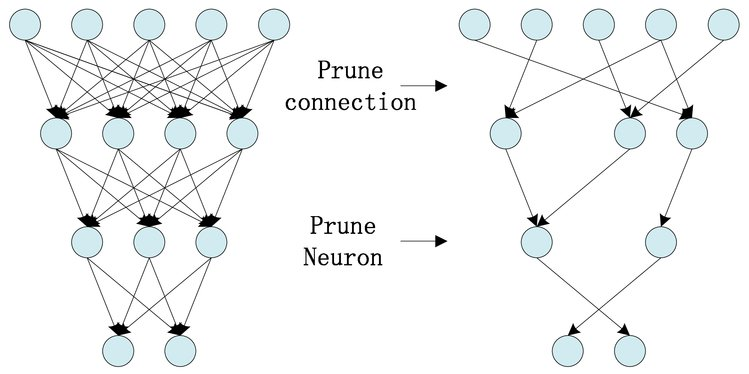
\includegraphics[width=0.65\linewidth]{fig/pruning.jpg}
	\caption{CNN voor en na pruning}
	\label{fig:pruning}
\end{figure}

\subsection{Parameter kwantisatie}
Het kwantiseren van gewichten is een tweede methode voorgesteld door \cite{han_deep_2016}.
Een CNN bestaat uit miljoenen gewichten en de waarde van elke van deze gewichten moet op het systeem worden opgeslagen.
De defaultrepresentatie van een waarde wordt opgeslagen als een floating point wat 4 bytes in beslag neemt.
Dus voor miljoenen parameters hebben de gewichten veel schijfruimte nodig.
Een mogelijke oplossing hiervoor is het kwantiseren van gewichten.
Hierbij wordt de getalrepresentatie van de gewichten verandert naar een representatie die minder geheugen in beslag neemt, een voorbeeld is te zien op figuur \ref{fig:kwantizatie}.

\begin{figure}[!ht]
	\centering
	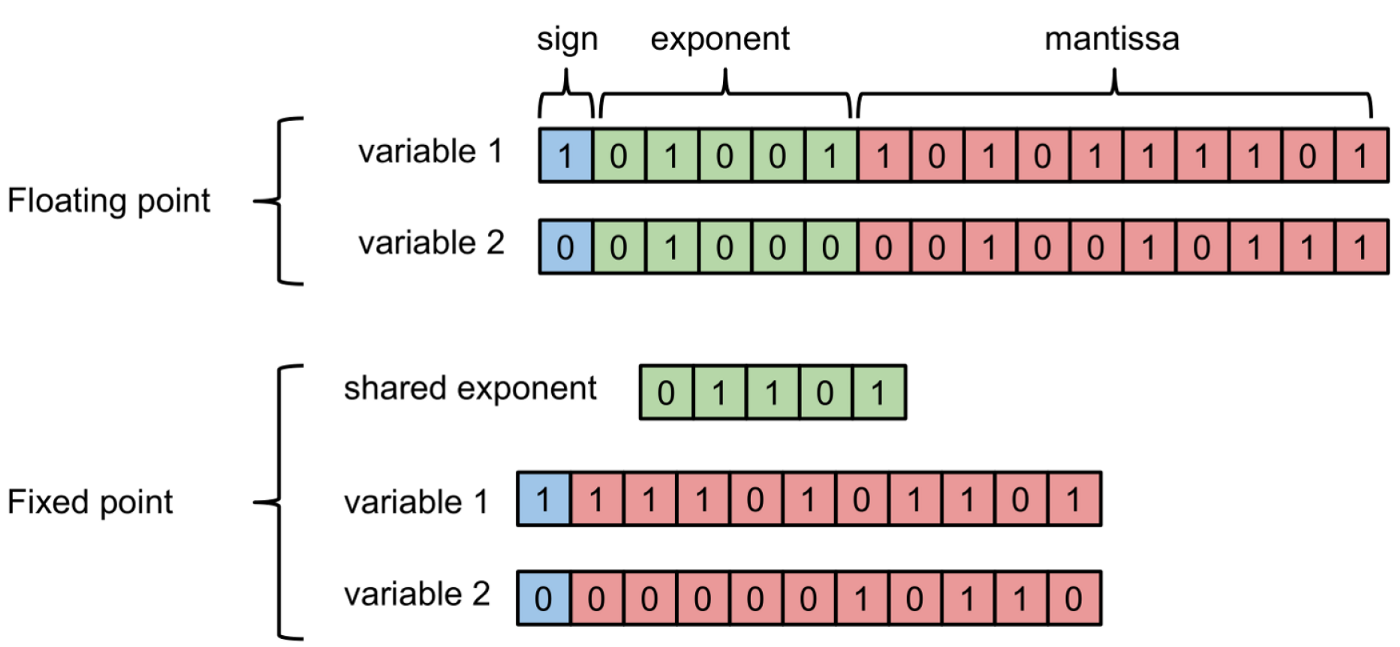
\includegraphics[width=0.7\linewidth]{fig/kwantization.png}
	\caption{kwantisatie van twee floating piont variabelen die worden omgezet naar twee fixed point variabelen met een gemeenschappelijke exponent.}
	\label{fig:kwantizatie}
\end{figure}

\subsection{Weight Clustering}
Hierbij worden de waarden van gewichten beperkt tot een set van beschikbare waardes (\cite{han_deep_2016}) dit is te zien op figuur \ref{fig:clus}.
Waarbij de waardes eenmalig worden opgeslagen en al de gewichten refereren naar een waarde van de vaste set met waardes.
Hoe kleiner de set met waardes is hoe minder geheugen er in beslag wordt genomen, maar een kleinere set van waardes zorgt ook voor een mindere accuratie.
\cite{han_deep_2016} past vervolgens Huffman encodering toe die een compressie uitvoert op de geclusterde parameters.

\begin{figure}[!ht]
	\centering
	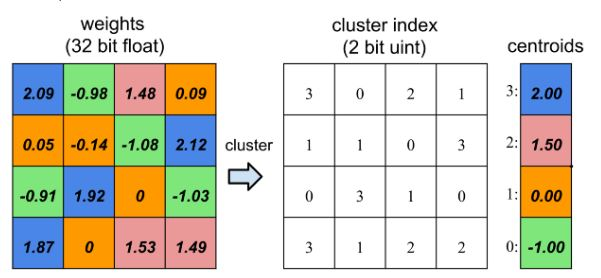
\includegraphics[width=0.7\linewidth]{fig/clus.jpg}
	\caption{Weight clustering: links zijn allemaal verschillende gewichten en na het het uitvoeren van weight clustering zijn er in de matrix pointers terug te vinden die wijzen kunnen wijzen naar vier verschilende waarden.}
	\label{fig:clus}
\end{figure}

\subsection{Convolutionele filter compressie en matrix factorisatie}
Een andere methode voorgesteld is Compressed Convolutional Filters (\cite{goel_survey_2020}).
Hierbij wordt de grootte van de kernel verkleind om het aantal parameters en rekenwerk te verminderen.
Maar door de kernels te verkleinen daalt de accuraatheid van het CNN.
Bij matrix factorisatie (\cite{goel_survey_2020}) worden grootte en complexe matrices opgesplitst in verschillende kleinere en eenvoudigere matrices.
Op deze manier worden ook redundante operaties uit het model gefilterd.


%%%%%%%%%%%%%%%%%%%%%%%%%%%%%%%%%%%%%%%%%%%%%%%%%%%%%%%%%%%%%%%%%%% 
%                                                                 %
%                            CHAPTER                              %
%                                                                 %
%%%%%%%%%%%%%%%%%%%%%%%%%%%%%%%%%%%%%%%%%%%%%%%%%%%%%%%%%%%%%%%%%%% 
\chapter{Experimenten}
\section{Converteren naar framework voor mobiele implementatie}
Het doel van deze masterproef is om een bestaand netwerk op een mobiel platform te krijgen.
Dus zullen de detectoren die ontworpen zijn in TensorFlow en PyTorch geconverteerd moeten worden naar een framework voor mobiele implementatie.
Voor het ontwerpen van detectoren kan er gebruik gemaakt worden van bibliotheken: Detectron2, MMDetection, ImagAI en GluonCV die vermeld zijn in paragraaf \ref{lib}.
Maar dit kan het converteren meer complex maken.
Omdat deze bibliotheken gebruik kunnen maken van operaties die niet compatibel zijn met het gewenste framework.
Detectoren zijn complexe systemen waarbij het converteren naar een ander framework complex of zelfs niet mogelijk zal worden.
In deze paragraaf zal er voor de MMDetection bibliotheek gekeken worden wat de mogelijkheden zijn om van een detector model naar een mobiele implementatie te gaan.
De eerste stap zal zijn om te kijken welke mogelijkheden er zijn zonder te converteren naar een ander framework.
Een tweede stap is via ONNX het huidige detectiemodel converteren naar een andere framework.
Een derde stap is verder zoeken naar een alternatief als de eerste twee methodes niet lukken.

Voor het testen van MMDetection nemen we de Kitty dataset \cite{Geiger_IJRR_2013} die bestaat uit auto's en voetgangers waarmee we een detector trainen via transfer learning.
Voor de basisdetector nemen we een voorgetraind Faster-RCNN detector.

\subsection{Van MMDetection model naar PyTorch Mobile model} \label{pmob}
Vermits MMDetection bovenop PyTorch werkt is de meest voor de hand liggende techniek om via PyTorch Mobile een model te genereren.
Voordat het model kan geoptimaliseerd worden moet het pythonafhankelijk model worden omgezet in TorchScript. 
Deze TorchScript module kan dan verder geoptimaliseerd worden voor mobiel gebruik.
Het omzetten naar de scriptmodule geeft de volgende Error: \newline
\textcolor{red}{TypeError: forward() missing 1 required positional argument: 'img\_metas'} \newline
Dit probleem is mogelijks op te lossen door de 'example' input aan te passen naar een gepaste input Tensor.
Op deze manier kan de jit.trace functie het model uitvoeren met de correcte input.

\subsection{Van MMDetection model naar ONNX model}
Voor gebruik te maken van andere frameworks voor mobiele implementatie zal het model eerst geconverteerd moeten worden naar ONNX formaat.
MMDetection ondersteunt de conversie naar ONNX, dit zit nog in zijn experimentele fase en MMDetection ondersteund momenteel enkel opset-versie 11 van ONNX.
In de documentatie van MMDetection kan er een lijst gevonden worden met detectiemodellen die ondersteuning hebben voor het exporteren naar ONNX.
MMDetection gebruikt een eigen script om een model te exporteren naar ONNX.
Via de volgende lijn code is het mogelijk om het MMDetection model om te zetten naar een ONNX model.

\begin{python}
python ./tools/deployment/pytorch2onnx.py <config_file> <checkpiont_file> 
	--output-file <output file>
\end{python}

pytorch2onnx.py is het MMDetection script om een model te converteren naar ONNX formaat.
De config file is het bestand dat het neuraal netwerk beschrijft.
En de checkpoint file is het model zelf dat tijdens het trainen wordt aangemaakt.
Het finale model is normaal gezien terug te vinden als latest.pth, dit is het laatste checkpoint dat tijdens het trainen wordt aangemaakt.
Op het einde van deze lijn code is het mogelijk om nog extra opties toe te voegen die in de MMDetection documentatie terug te vinden zijn.
Dit script gebruikt geen nieuwe methode om naar ONNX te converteren, maar maakt gebruik van de ONNX export functie van pytorch.
Bovenstaande lijn code converteert het Faster-RCNN model succesvol naar een ONNX model.
Wel moet er bij vermeld worden dat dit MMDetection model een standaardmodel is waarbij geen specifieke aanpassingen zijn gedaan.
Dus bij complexere modellen zou het resultaat anders kunnen zijn.
Doordat we nu een ONNX model hebben zijn er een aantal nieuwe mogelijkheden om het model te implementeren op een mobiel apparaat.

\subsection{Van ONNX model naar mobiele implementatie}
We kunnen het ONNX model omzetten naar een onnxruntime model, maar bij het implementeren van onnxrunime model in Android studio krijgen we de volgende error: \newline
\textcolor{red}{'java.lang.UnsatisfiedLinkError: No implementation found for long ai.onnxruntime.\newline
.createOptions(long) tried Java\_ai\_onnxruntime\_OrtSession\_00024SessionOptions\newline
\_createOptions and Java\_ai\_onnxruntime\_OrtSession\_00024SessionOptions\_createOptions\_J'} \newline
Deze error onststaat wanneer de applicatie een bibliotheek probeert in te laden, maar deze bibliotheek bestaat niet.
Zowel de standaardbibliotheek als de onxxruntime-mobile bibliotheek geven deze fout.
Een mogelijke oplossing zou zijn om de correcte bibliotheek handmatig toe te voegen aan Android studio.

Het ONNX model implementeren in javascript werd daarentegen wel uitgevoerd zonder fouten.

\subsection{Van ONNX model naar TensorFlow model}
Met het gegenereerde ONNX model is het mogelijk om het model om te zetten naar een TensorFlow model en vervolgens naar een TFLite model om te zetten.
Hierbij komen al 3 conversies aan te pas en met elke conversie dus is de kans groter dat het uiteindelijke model een error geeft.
Het converteren van een .onnx bestand naar een TensorFlow Lite model kan met behulp van de volgende lijnen code.

\begin{python}
import tensorflow as tf
import onnx
from onnx_tf.backend import prepare
	
#ONNX model inladen 
onnx_model = onnx.load("model.onnx")  # inladen onnx model
output = prepare(onnx_model)
output.export_graph('tf_model.pb') # model exporteren naar TensorFlow model

#Ingeladen model omzetten naar TensorFlow Lite model
converter = tf.lite.TFLiteConverter.from_saved_model('tf_model.pb')
converter.target_spec.supported_ops = [
	tf.lite.OpsSet.TFLITE_BUILTINS, # enable TensorFlow Lite ops.
	tf.lite.OpsSet.SELECT_TF_OPS # enable TensorFlow ops.
]
tflite_model = converter.convert() # converteer model
\end{python}

Eerst moet het ONNX model ingeladen worden als een standaard TensorFlow model.
Vervolgens moet bij het converteren naar een TensorFlow Lite model eerst vermeld worden welke TensorFlow operaties ondersteund moeten worden.
Het effectief converteren naar een TensorFlow Lite model duurde ongeveer 30 minuten voor dit testmodel.
bij het uitvoeren van dit model in Android studio krijgen we de volgende error: \newline
\textcolor{red}{'java.lang.AssertionError: Error occurred when initializing ObjectDetector: Didn't find op for builtin opcode 'MUL' version '5'. An older version of this builtin might be supported. are you using an old TFLite binary with a newer model.'}\newline
Deze fout geeft aan dat de 'MUL' operatie niet ondersteund wordt door TensorFlow.
Om dit probleem op te lossen zouden we kunnen zoeken naar een TFLite versie die deze operatie wel ondersteund.
We zouden ook kunnen proberen om deze opperatie te vervangen door een opperatie die wel ondersteund wordt.

\subsection{Converteren naar CoreML model}
Bij het converteren naar CoreML vanuit PyTorch stoten we op hetzelfde probleem als bij het converteren naar PyTorch Mobile in paragraaf \ref{pmob}.
De tweede manier om naar CoreML te gaan is vanuit TensorFlow, maar dit is een vrij omslachtige manier omdat we dan de volgende conversies moeten maken MMDetection \textrightarrow ONNX \textrightarrow TensorFlow \textrightarrow CoreML. 
Maar om van TensorFlow naar CoreML te gaan verwacht de converter een Keras model, maar dit is er niet vermits het model in MMDetection is ontworpen.

\subsection{Conclusie}
Om van een MMDetection model naar een mobiele implementatie te gaan is een complex process dat op een aantal problemen stoot.
Geen enkel model werd na het converteren succesvol uitgevoerd.
De enige methode waarbij het model werd uitgevoerd is de onnxruntime implementatie in javascript.
We zijn hier vertrokken vanuit een complex geval en we zijn op heel wat problemen gestoten.
Voor toekomstige experimenten gaan we vertrekken vanuit een eenvoudig geval.
En we gaan dit steeds verder uitbreiden zodat we kunnen zien waar we exact op een probleem stoten.
Op deze manier kunnen we het probleem dan eenvoudiger oplossen.
%%%%%%%%%%%%%%%%%%%%%%%%%%%%%%%%%%%%%%%%%%%%%%%%%%%%%%%%%%%%%%%%%%% 
%                                                                 %
%                            CHAPTER                              %
%                                                                 %
%%%%%%%%%%%%%%%%%%%%%%%%%%%%%%%%%%%%%%%%%%%%%%%%%%%%%%%%%%%%%%%%%%% 
\chapter{Richtlijnen voor referenties}

\section{Inleiding}
De referentielijst bevat de volledige lijst van literatuur en bronnen waarnaar in de tekst wordt verwezen. Door systematisch de referentielijst aan te vullen bij het schrijven van het literatuuroverzicht gaat er achteraf geen tijd verloren aan het opnieuw opzoeken van referenties.

\section{Referentiestijl}

Voor het verwijzen naar informatiebronnen wordt gebruik gemaakt van het numerisch systeem  of van het auteur-jaar systeem. Dit kies je door volgend commando in het latex bronbestand aan te passen:

\begin{itemize}
	\item numerisch (IEEE) : \verb|\bibliographystyle{ieee}|
	\item alfabetisch (APA) : \verb|\bibliographystyle{apalike}|
\end{itemize}

Plaats je bronnen in een \textit{bibtex} bestand (evt. via software zoals bv. Jabref Endnote of Mendeley), waarnaar je verwijst vanuit je thesis text a.d.h.v. het commando \verb|\cite|. Enkele links naar nuttige software in deze context:

\begin{itemize}
	\item \href{http://www.jabref.org/}{JabRef (Open Source)}
	\item \href{http://www.mendeley.com}{Mendeley (Freeware)}
	\item \href{http://www.endnote.com}{EndNote (Paid license)}
\end{itemize}

Indien je zelf een .bibtex bestand wil aanleggen dien je volgende syntax te volgen voor een tijdschriftartikel:
\clearpage
\verb|@article{hughes2005,|\\
\verb|title={Isogeometric analysis: CAD, finite elements, NURBS, exact geometry|\\ \verb|and mesh refinement},|\\
\verb|author={Hughes, Thomas JR and Cottrell, John A and Bazilevs, Yuri},|\\
\verb|journal={Computer methods in applied mechanics and engineering},|\\
\verb|volume={194},|\\
\verb|number={39},|\\
\verb|pages={4135--4195},|\\
\verb|year={2005},|\\
\verb|publisher={Elsevier}|\\
\verb|}|

Enkele voorbeelden van het gebruik van bronnen in een tekst (in APA stijl): 

Recent werd het Higgs boson experimenteel vastgesteld door Aad et al.\ \cite{aad2012} (syntax: \verb|\cite{aad2012}|). 

Als alternatief voor het discretiseren van een CAD model vooraleer een eindige elementenanalyse te kunnen toepassen, stellen Hughes et al.\ voor om de nodige elementenformulering rechtstreeks uit de NURBS beschrijving van de CAD geometrie te halen \cite{hughes2005} (syntax: \verb|\cite{hughes2005}|). Daarnaast introduceren ze tevens een k-iteratieve procedure als een verfijning van de geldende p- en h-iteratieve procedures in eindige elementen methoden \cite{cottrell2009} (syntax: \verb|\cite{cottrell2009}|).
% Bibliografie: referenties. De items zitten in bibliografie.bib
%%%%%%%%%%%%%%%%%%%%%%%%%%%%%%%%%%%%%%%%%%%%%%%%%%%%%%%%%%%%%%%%%
% Indien je ook de niet geciteerde werken in je bibliografie wil opnemen, commentarieer dan onderstaande regel uit!
%\nocite{*}
\bibliographystyle{apalike}
\bibliography{bibliografie}

% Eventueel enkele appendices
%%%%%%%%%%%%%%%%%%%%%%%%%%%%%%
\appendix
\chapter{Uitleg over de appendices}
Bijlagen worden bij voorkeur enkel elektronisch ter beschikking gesteld. Indien essentieel kunnen in overleg met de promotor bijlagen in de scriptie opgenomen worden of als apart boekdeel voorzien worden.

Er wordt wel steeds een lijst met vermelding van alle bijlagen opgenomen in de scriptie. Bijlagen worden genummerd het een drukletter A, B, C,...

Voorbeelden van bijlagen:\\
Bijlage A: \qquad	Detailtekeningen van de proefopstelling \\
Bijlage B: \qquad	Meetgegevens (op USB)
\\





% Back cover: change according to the correct campus

\includepdf{private/back_fiiw_denayer.pdf}
% 
\includepdf{private/back_fiiw_denayer_eng.pdf} % For the english version
%
\includepdf{private/back_fiiw_geel.pdf}
% 
\includepdf{private/back_fiiw_geel_eng.pdf} % For the english version
%
\includepdf{private/back_fiiw_gent.pdf}
% 
\includepdf{private/back_fiiw_ghent_eng.pdf} % For the english version
%
\includepdf{private/back_fiiw_brugge.pdf}
% 
\includepdf{private/back_fiiw_bruges_eng.pdf} % For the english version
%
\includepdf{private/back_fiiw_groept.pdf}
% \includepdf{private/back_fiiw_groupt_eng.pdf} % For the english version

\end{document}
